\def\year{2020}\relax
%File: formatting-instruction.tex
\documentclass[letterpaper]{article} % DO NOT CHANGE THIS
\usepackage{aaai20}  % DO NOT CHANGE THIS
\usepackage{times}  % DO NOT CHANGE THIS
\usepackage{helvet} % DO NOT CHANGE THIS
\usepackage{courier}  % DO NOT CHANGE THIS
\usepackage[hyphens]{url}  % DO NOT CHANGE THIS
\usepackage{graphicx} % DO NOT CHANGE THIS
\urlstyle{rm} % DO NOT CHANGE THIS
\def\UrlFont{\rm}  % DO NOT CHANGE THIS
\usepackage{graphicx}  % DO NOT CHANGE THIS
\frenchspacing  % DO NOT CHANGE THIS
\setlength{\pdfpagewidth}{8.5in}  % DO NOT CHANGE THIS
\setlength{\pdfpageheight}{11in}  % DO NOT CHANGE THIS
%\nocopyright
%PDF Info Is REQUIRED.
% For /Author, add all authors within the parentheses, separated by commas. No accents or commands.
% For /Title, add Title in Mixed Case. No accents or commands. Retain the parentheses.
 \pdfinfo{
/Title (ARO:  A Memory-Based Approach to Environments with State Aliasing)
/Author (Ryan Regier, Owen Price, Alex Hadi, Zachary Faltersack and Andrew Nuxoll)
} %Leave this	
% /Title ()
% Put your actual complete title (no codes, scripts, shortcuts, or LaTeX commands) within the parentheses in mixed case
% Leave the space between \Title and the beginning parenthesis alone
% /Author ()
% Put your actual complete list of authors (no codes, scripts, shortcuts, or LaTeX commands) within the parentheses in mixed case. 
% Each author should be only by a comma. If the name contains accents, remove them. If there are any LaTeX commands, 
% remove them. 

% DISALLOWED PACKAGES
% \usepackage{authblk} -- This package is specifically forbidden
% \usepackage{balance} -- This package is specifically forbidden
% \usepackage{caption} -- This package is specifically forbidden
% \usepackage{color (if used in text)
% \usepackage{CJK} -- This package is specifically forbidden
% \usepackage{float} -- This package is specifically forbidden
% \usepackage{flushend} -- This package is specifically forbidden
% \usepackage{fontenc} -- This package is specifically forbidden
% \usepackage{fullpage} -- This package is specifically forbidden
% \usepackage{geometry} -- This package is specifically forbidden
% \usepackage{grffile} -- This package is specifically forbidden
% \usepackage{hyperref} -- This package is specifically forbidden
% \usepackage{navigator} -- This package is specifically forbidden
% (or any other package that embeds links such as navigator or hyperref)
% \indentfirst} -- This package is specifically forbidden
% \layout} -- This package is specifically forbidden
% \multicol} -- This package is specifically forbidden
% \nameref} -- This package is specifically forbidden
% \natbib} -- This package is specifically forbidden -- use the following workaround:
% \usepackage{savetrees} -- This package is specifically forbidden
% \usepackage{setspace} -- This package is specifically forbidden
% \usepackage{stfloats} -- This package is specifically forbidden
% \usepackage{tabu} -- This package is specifically forbidden
% \usepackage{titlesec} -- This package is specifically forbidden
% \usepackage{tocbibind} -- This package is specifically forbidden
% \usepackage{ulem} -- This package is specifically forbidden
% \usepackage{wrapfig} -- This package is specifically forbidden
% DISALLOWED COMMANDS
% \nocopyright -- Your paper will not be published if you use this command
% \addtolength -- This command may not be used
% \balance -- This command may not be used
% \baselinestretch -- Your paper will not be published if you use this command
% \clearpage -- No page breaks of any kind may be used for the final version of your paper
% \columnsep -- This command may not be used
% \newpage -- No page breaks of any kind may be used for the final version of your paper
% \pagebreak -- No page breaks of any kind may be used for the final version of your paperr
% \pagestyle -- This command may not be used
% \tiny -- This is not an acceptable font size.
% \vspace{- -- No negative value may be used in proximity of a caption, figure, table, section, subsection, subsubsection, or reference
% \vskip{- -- No negative value may be used to alter spacing above or below a caption, figure, table, section, subsection, subsubsection, or reference

\setcounter{secnumdepth}{0} %May be changed to 1 or 2 if section numbers are desired.

% The file aaai20.sty is the style file for AAAI Press 
% proceedings, working notes, and technical reports.
%
\setlength\titlebox{2.5in} % If your paper contains an overfull \vbox too high warning at the beginning of the document, use this
% command to correct it. You may not alter the value below 2.5 in
\title{ARO:  A Memory-Based Approach to Environments with State Aliasing }
%Your title must be in mixed case, not sentence case. 
% That means all verbs (including short verbs like be, is, using,and go), 
% nouns, adverbs, adjectives should be capitalized, including both words in hyphenated terms, while
% articles, conjunctions, and prepositions are lower case unless they
% directly follow a colon or long dash


\author{Author's Names Omitted for Peer Review
%% \author{Ryan Regier, Owen Price, Alex Hadi, Zachary Faltersack and Andrew Nuxoll \\ 
%% University of Portland\\ %If you have multiple authors and multiple affiliations
%% 5000 North Willamette Boulevard\\
%% Portland, Oregon 97203\\
%% engineering@up.edu % email address must be in roman text type, not monospace or sans serif
}


%%%%%%%%%%%%%%%%%%%%%%%%%%%%%%%%%
% Ryan's packagages

\usepackage{algorithmicx} % Used for writing algorithms
\usepackage{algpseudocode} % Default algorithm psedocode for algorimicx
\usepackage{comment}
%%%%%%%%%%%%%%%%%%%%%%%%%%%%%%%%%
 \begin{document}

\maketitle

\begin{abstract}
Episodic memory, or the ability to remember specific events from your
past, is an essential part of human cognition.  While most machine
learning tasks do not require this capability, episodic memory is
essential is learning in environments with severe state aliasing
(a.k.a., perceptual aliasing).  In this paper we define two specific
environments with severe state aliasing and then present ARO, an
algorithm for learning in such an environment.  Our results show that
ARO is effective where traditional algorithms would fail.
\end{abstract}

\noindent


The foundation of this work is in research towards an artificial,
general episodic memory.  Episodic memory is one of three, long term
memories commonly recognized in humans \cite{Tulving83}.  Evidence
from psychology research indicates that an impaired ability to form
new episodic memories (i.e., anterograde amnesia) also impairs
learning \cite{Brooks76}.  Furthermore, common sense tells us
that possesing a memory of past experiences is essential to a number
of fundamental cognitive capabilities including our own sense of
identity \cite{Holland10,Nuxoll12}.

Thus, we believe it behooves those who wish to create an artificial
general intelligence to seek to create algorithms that possess and
leverage an artificial, general episodic memory.  An artificial episodic
memory has been applied to a number of specific environments.
ee \cite{Tecuci07,Brom08,Castro10,Chaudhry18} for a sample.  We know
of only a few existing approaches to a general artificial episodic
memory in part of a broad, general
architecture \cite{Boloni11,Nuxoll12,Menager16}.




\section{Extreme State Aliasing}
To learn about effective episodic learning, we seek to create
environments where an agent's episodic memory is essential for
success.  One such environment is the Blind Finite State Machine
environment.  In this environment, the agent navigates a finite state
machine (FSM) \cite{Hopcroft06} to reach a goal state.  The machine is
designed so that the agent can reach the goal from any state (no dead
ends) but otherwise the transition table is randomly generated.  Upon
reaching the goal the agent is immediately moved to a randomly
selected, non-goal state and informed of its success.  Thus the agent
knows when it reaches the goal but can never actually take an action
in the goal state.

The task seems trivial at first.  However, it is greatly complicated
because the agent is only aware of the following:
\begin{itemize}
\item the FSM alphabet (available actions)
\item a goal sensor indicating when it reaches the goal
\end{itemize}

\bigskip  %vertical space here makes this more readable

Specifically, the agent is \underline{not} aware of the following:
\begin{itemize}
\item the number of states
\item what state it currently is in
\item the transition table of the FSM
\end{itemize}

The agent repeatedly performs the task in a given FSM and its success
is measured by how many states it takes to reach the goal at each
iteration.  Experiments with human subjects (not published) indicate
that this task is exceptionally difficult for humans.

In such an environment, a traditional machine learning agent is unable
to learn effective behavior.  Such an agent attempts to learn the
action that yields the maximum expected utility for each possible
sensory input.  However, in this environment, all states (except the
goal state) appear identical to the agent.  So, the agent can only
learn a single ``best'' action to take in any non-goal state.

To be successful in the Blind FSM environment, an agent must map
\textit{sequences of episodes} to actions where an episode is in this
case as the agent's sensory input and the action it selected.  For
example, the agent can learn if it takes actions $a_1, a_2, ..., a_n$
in sequence and does not reach then goal that it can subsequently
reach the goal in a single step by taking action $a^*$.  Furthermore,
the agent can learn that certain sequences of actions have more
utility than others regardless of what non-goal state it is currently
in.

To learn effective sequences of episodes, an agent must have an
episodic memory.  Specifically, a memory of previous episodes allows
the agent to identify its current state and/or successful sequences of
actions.

In previous research, an algorithm called MaRz \cite{Rodriguez17} has
shown the best success in Blind FSM environments.  MaRz performs an
A*-Search \cite{Russell09}over possible sequences of actions to find
the shortest \textit{universal sequence}.  A universal sequence is a
sequence of actions that causes the agent to reach the goal from any
non-goal state.  For example, consider the state machine in
Figure \ref{fig1}.

\begin{figure}[t]
\centering
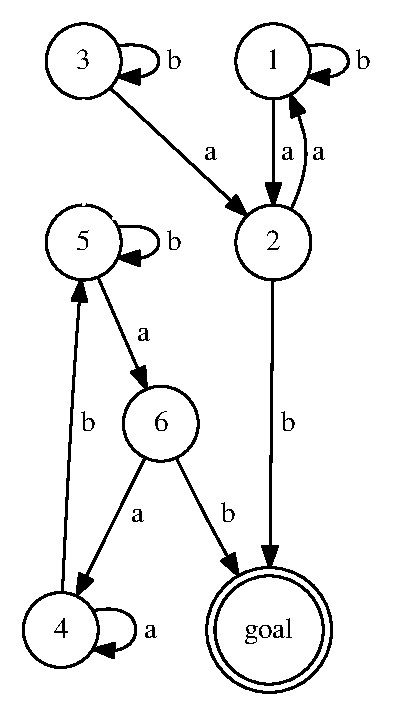
\includegraphics[width=0.6\columnwidth]{ExampleFSM} % Reduce the figure size so that it is slightly narrower than the column. Don't use precise values for figure width.This setup will avoid overfull boxes. 
\caption{An example Blind FSM}
\label{fig1}
\end{figure}


%  Here is the transition table for the FSM in the figure
%          a  b
%       1  2  1
%       2  1  G
%       3  2  3
%       4  4  5
%       5  6  5
%       6  4  G

The agent begins in a random, non-goal state.  It first takes action
'b' and does not reach the goal as a result of this action.  While the
agent does not know the transition table of the FSM, we can look at
the diagram and know that the agent must have begun in state 1, 3, 4
or 5 and now must be in state 1, 3 or 5.  As a result, we know that
the agent is guaranteed to reach the goal in two steps if it takes the
action \textit{a} followed by \textit{b}.  This makes \textit{bab} a
universal sequence for this particular FSM.

\section{A Little Less State Aliasing}

% Do we need to discuss the lack of tuning parameters?

The situation changes once the agent is given additional sensors
beyond the goal sensor.  Consider an environment like Blind FSM but
the agent also has a binary sensor that tells it when it is currently
in an odd state or an even state.  We shall henceforth refer to this
as the OSFSM (Odd-Sensor Finite State Machine) environment.

For an OSFSM environment using the FSM in Figure \ref{fig1}, the
universal sequence (\textit{bab}) is sub-optimal.  The agent can
consistently reach the goal faster (or at least as fast) by always
taking action \textit{b} in even numbered states and action \textit{a}
in odd numbered states.  Thus, the MaRz algorithm needs to be enhanced
or replaced in such situations.

An episodic memory remains essential to be successful in the OSFSM
environment.  Traditional machine learning algorithms still perform
poorly in OSFSM since they can still only ever distinguish three
states.  However, as more and more sensors are provided a traditional
machine learning algorithm becomes more and more effective.  Thus,
there is a continuum from complete state aliasing (e.g., the Blind FSM
environment) to a fully observable environment.

The goal becomes to create an algorithm that can function well in
both.  This research presents ARO, an initial step toward such an
algorithm.

\section{Environment}

We formally classify the environment for ARO. We define the environment by a tuple $(G, M, O, f)$. The machine $M$ is a finite state machine with state set $S$, alphabet $\alpha$, and transition function $T$ such that the goal state $G$ is in $S$ and there is a path from every state in $S$ to $G$. The observation set $O$ is the set of possible observations (different sensor values) where $G \in O$ denotes the observation of the goal state. The observation function $f: S \rightarrow O$ computes what is observed in any state where $f(s) = G$ if and only if $s = G$. 

An agent in this environment is told $\alpha$, but is otherwise provided no information about the environment. At any time-step $t$ when the agent is in state $s_t$, the agent will be told $f(s_t)$. If $s_t$ is not a goal state, the agent must provide an action $a_t \in \alpha$. The agent will then transition to $s_{t+1} = T(s_t, a_t)$. If $s_t$ is a goal state, the agent will be moved to non-goal state $s_{t+1}$ at random. This will continue until an arbitrary but unknown number of goals are reached. The goal of the agent is to minimize the total number of time steps.

In the Blind FSM environment, $O = \{\epsilon, G\}$ and $f(s) = \epsilon$ for non-goal states. In the OSFSM environment, $O = \{0, 1, G\}$, with $0$ and $1$ denoting whether the state is even or odd, respectively, and $f(s)$ returns the parity of s for non-goal states.

\section{ARO Overview}

%ARO can be described in three parts: a data structure to store episodic memories and to describe what is currently known about the position of the agent in the machine, a method to estimate the value of exploring vs exploiting based on the data gathered, and an algorithm to use the data structure and the explore-exploit heuristic to decide what action to perform.

\subsection{Data Structures}

We begin with data structures used for ARO. The agent stores previous events in atomic units called ``episodes." Each episode consists of the tuple $(o, a)$, where $o$ is the observation ($f(s)$), and $a$ is the action taken after the observation. In the OSFSM environment, an example episode may be $(1,b)$. When the agent reaches the goal, no action is performed, so we denote such an episode simply with ``G." In non-goal episodes, we concatenate the tuple for brevity, so the above episode would be denoted ``1b". In this episode, the agent was in an odd state and took action $b$.

Using these episodic memories, the agent records patterns of cause and effect in a structure called a ``rule." Rules are denoted like this example: $$1a \rightarrow 1: 23\%.$$ This rule states that being in an odd state and taking action $a$ ``caused" an odd state $23\%$ of the time. The effect part of a rule is always in this same style, but causes may be more complex. For example, consider this rule: $$0b,1a \rightarrow 1: 6\%.$$ This rules says that the agent taking action $a$ while being in an odd state that was reached by taking a $b$ from an even state has caused an odd state $6\%$ of the time. In general, a rule consists of a sequence of episodes as the ``cause", an observation $o \in O$ as an ``effect," and the probability that the cause produces the stated effect. The cause sequence of a rule may be empty, which can be interpreted as the probability  that transitioning to a new state causes a particular observation. The number of episodes in the cause sequence of a rule is called the ``depth" of a rule.

The authors used a tree data structure to store rules, but this choice does not effect functionality. So rather than explain this tree, we merely define the function \scshape GetRule\normalfont that takes as inputs both a cause sequence and a effect then produces as an output the corresponding rule. We also define ``rule group" as the set of all rules with the same cause sequence and the function \scshape GetRuleGroup \normalfont that takes as an input a cause sequence and produces as an output the corresponding rule group.

%There are multiple rules with the same cause sequence. For instance, both $1a \rightarrow 0: 3$ and $1a \rightarrow G: 2$ may be rules. By comparing all rules with the same cause sequence, the agent can compute the probability that any particular effect will occur. We will call this set of rules a ``rule group." We define the function called \scshape GetRuleGroup\normalfont(episodes), which takes an array of episodes and returns the corresponding rule group.

%For a given sequence of episodes, many rule groups apply. For example, the sequence $1a,0a,1b$ has 4 rule groups apply: the group for the full sequence, the $0a,1b$ group, the $1b$ group, and the group for the empty sequence. Each will produce different probabilities of what will be observed next. The probabilities from the high-depth groups will be less accurate due to having less data, but can describe more sophisticated patterns than low-depth groups. The array of rule groups that currently apply is called ``current."

Now that we have a method for storing patterns of cause and effect, we can use this information in the agent's memory to predict future outcomes and find the optimal move.

\subsection{Expected Value}

Given a sequence of previous episodes that have occurred and an observation, we can recursively compute the expected number of moves it will take to reach the goal. This is computed under the assumption that at each choice the agent may have in the future, it will make the best possible move. The algorithm is below.

\begin{comment}
\begin{algorithmic}[1]
	\Function{ExpectedValue}{RuleGroup $group$}
		\State $Sum = 0$
		\For{$rule$ in $group$}
			\State Let $p$ be the probability of $rule$ occurring.
			\State Let $e$ be the effect of $rule$.
			\If{$e = G$}
				\State $Sum = Sum + p$
			\Else
				\State Let $episodes$ be the cause sequence of $rule$
				\For{$a$ in $\alpha$}
					\State Let $next = (e, a)$ be a new episode.
					\State Let $nextSequence$ be the array $episodes$ appended by $next$
					\State $nextGroup =$ \Call{GetRuleGroup}{$nextSequence$} % Note: This looks awful because LaTeX spreads out spacing. This will need the full page to loook correct
					\State $Sum = Sum \ + p*($ \Call{ExpectedValue}{$nextGroup$} $ + 1)$
				\EndFor
			\EndIf
		\EndFor
	\EndFunction
\end{algorithmic}
\end{comment}


\begin{algorithmic}[1]
	\Function{ExpectedValue}{Episode[] $episodes$, Observation $o$}
		\State $BestSum = \infty$
		\State $BestMove = \epsilon$
		\For{$a$ in $\alpha$}
			\State $Sum = 0$
			\State Let $next = (o, a)$ be a new episode.
			\State Let $nextSequence$ be $episodes$ appended by $next$
			\State $nextGroup =$ \Call{GetRuleGroup}{$nextSequence$} % Note: This looks awful because LaTeX spreads out spacing. This will need the full page to loook correct
			\If{$nextGroup$ is empty}
				\State $Sum = $ \Call{GetHeuristic}{~} \label{line:heuristic}
			\EndIf
			\For{$rule$ in $nextGroup$}
				\State Let $e$ be the effect of $rule$.
				\State Let $p$ be the probability of $rule$.
				\If{$e = G$}
					\State $Sum = Sum + p$
				\Else
					\State $Sum = Sum + p*($\Call{ExpectedValue}{$nextSequence$, $e$} $ + 1)$
				\EndIf
			\EndFor
			\If{$Sum < BestSum$}
				\State $BestSum = Sum$
				\State $BestMove = a$
			\EndIf
		\EndFor
	\State \Return $BestSum$
	\EndFunction
\end{algorithmic}

This algorithm also computes the move that will take the fewest number of steps to reach the goal on average, stored in the $BestMove$ variable. Let \scshape GetBestMove \normalfont be a function that, when given the same inputs as \scshape ExpectedValue \normalfont, will return the value of the $BestMove$ variable. The agent may call this function, supplying the most recent observation and an episode sequence ending at its most recent episode or an empty sequence. Thus, performing the action $BestMove$ can be used as a policy for the agent, and should minimize the average steps to goal based on what the agent has learned about the environment. In fact, this is exactly what ARO does. 

There are two aspects of this policy that are not yet well-defined. First, we cannot compute an expected value for a move we have never done before. This case is dealt with in line \ref{line:heuristic} of the code with the \scshape GetHeuristic \normalfont function that we have yet to describe. Second, there are multiple sequences the agent may pass into \scshape ExpectedValue \normalfont, from an empty sequence to the entire span of its episodic memory. Each sequence may produce a different expected value and recommended move to make, and the agent must choose which recommendation to follow. These are the corresponding topics of the next two sections.

\subsection{Explore Heuristic}
%Let us first deal with the case where we have no rules in a rule group and we must find the expected value. This occurs if the agent has never observed the sequence of episodes corresponding to the rule group. Let $e = (o, a)$ be the last episode in the rule group cause sequence and $seq$ be the rest of the sequence. This situation is equivalently described as follows: the agent has never recorded episodes in the sequence $seq$, then observed $o$ and performed action $a$. Thus, taking action $a$ can be considered an "exploration" by the agent. We therefore need to decide the value of exploring in this environment, which is clearly a bandit problem. Specifically, this is a contextual bandit problem with $seq$ and $o$ forming the context and the arms being the actions in $\alpha$. However, in this context
Let us first deal with the case where we must calculate an expected value when a rule group containing no rules. This can be equivalently stated as follows: there is an episode sequence $seq$ and observation $o$ where the agent has never performed action $a$. Thus, taking action $a$ can be thought of as an ``exploration" by the agent. We therefore need to decide the value of exploring in this environment in the units of expected value. While the explore-exploit tradeoff is well studied under the context of the Mulit-Armed Bandit problem and has several known solutions, we may use existing knowledge of this scenario to make a more specific solution.

It is possible to find an estimate of the expected value by using the rule group corresponding to removing the first episode from $seq$. However, repeating this process can lead to infinite depth recursion. Rather than creating a suitable base case to make the recursion finite, we instead attempted to estimate the value that this recursion will return. Let $p$ denote the probability of reaching the goal according to the $0$-deep rule group (that is, the probability corresponding to the rule $\_ \rightarrow G$). We note that if we were to continue recursion infinitely, the probability of reaching the goal in any step should converge on $p$. If we estimate that this probability holds constant on every step, then the number of steps to goal follows a Geometric distribution with probability $p$. This gives an expected value of $\frac{1}{p}$. Hence, we can now define the heuristic function:

\begin{algorithmic}[-1]
	
	\Function{GetHeuristic}{~}
		\State \Return $1/p$
	\EndFunction
	
\end{algorithmic}

TODO: DIVIDE BY 0!

As a benefit of this technique, we have derived a quantitative value of exploration without using hyperparameters, in contrast to traditional techniques for solving bandit problems such as $\epsilon$-greedy strategies or Q-learning. This fact makes this technique particularly suitable to online learning and artificial general intelligence problems where hyperparameter tuning is not possible or feasible. Also of note is that $\frac{1}{p}$ exactly equals the average number of steps to goal over the lifetime of the agent. (MENTION POKER?) This means that ARO's explore-exploit solution has an intuitive description: explore if the alternative is worse than average.

\subsection{Sequence Selection}

The agent may now calculate the best move given a sequence of recent episodes. However, different sized sequences may produce different results. With a large sequence, the episode sequence may be unique or rare in memory, producing poor results if the agent lacks knowledge regarding this specific context. Furthermore, a long sequence may contain superfluous information, which would imply that we are unnecessarily disregarding information from other, similar sequences. With a small sequence, the episode sequence may be too common for the agent to know where it is in the machine or to determine if it is going in a loop, which could cause undesirable behavior such as infinite looping. To resolve this dilemma, ARO uses the episode sequence that produces the smallest expected value. Hence, if the agent does have knowledge of a fast path to the goal from any valid context, it will take it. We expect this strategy to help reduce regret. If, on the other hand, the agent lacks useful knowledge of a quick path to a goal, it can fall back on a more reliable and average short sequence. This alone, however, is not sufficient to prevent loops.

At timestep $t$, say the sequence $seq$ has expected value $x$, and that this expected value was minimal. Hence, the action \scshape GetBestMove\normalfont($seq$) was performed. Let $nextSeq$ be $seq$ appended by the new episode generated by performing that action. We found that the expected value of $nextSeq$ in timestep $t+ 1$ can be higher than $x$, usually from an improbable event informing the agent that it is farther from the goal than the average case. When this occurred, the agent would switch to a shorter sequence for a move recommendation, which effectively ``forgets" that the agent is in a poor position. The agent then acts again like it is in an average position, which caused the agent to get stuck in a loop. To deal with this issue, we force the agent to deal with the bad event by not letting the agent switch to a different sequence for a move recommendation. In other words, if $seq$ was used to find  the best move at timestep $t$, then $nextSeq$ must be used to find the best move at timestep $t+1$. There are two exceptions to this rule. First, if the agent observes a goal. Because the agent is moved randomly upon reaching the goal state, there is no information to be gained by using a sequence with a goal observation. Second, if the agent discovers a new rule for which the current sequence is the cause sequence. This implies the agent is in a novel scenario and the current sequence can provide no data to guide the agent, so a new sequence must be selected to choose how to act.

Using these rules, we can now fully define the policy of ARO. We define the global variable $prevSequence$, which stores the sequence from the previous time step used to determine which action to take. ARO's policy is then described in the following algorithm.



\begin{algorithmic}
	
	\State Initialize $prevSequence$ to the empty sequence.

	\Function{Policy}{Observation $o$}
		\If{$o = G$}
			\State Set $prevSequence$ to the empty sequence.
			\State \Return
		\EndIf
		\State Let $e$ be the last episode.
		\State Let $seq$ be $prevSeq$ appended by $e$.
		\State Let $f$ be the frequency of $seq$ in episodic memory
		\If{$f = 1$ or $seq$ contains the episode $G$}
			\State Set $prevSeq$ to the sequence of recent episodes such that \Call{ExpectedValue}{$prevSeq$, $o$} is minimized.
			\State \Return \Call{GetBestMove}{$prevSeq$}
		\Else
			\State $prevSeq = seq$
			\State \Return \Call{GetBestMove}{$prevSeq$}
		\EndIf
		
	\EndFunction
	
\end{algorithmic}

%Often, it is necessary for the agent to look ahead more than one action. For example, if a rule group indicates to the agent that there is a $35\%$ chance that making an $a$ will lead to an odd state, it may be helpful to see what the chances are for reaching the goal by making an $a$ or $b$ from such an odd state. To allow for such operations, rules are stored in a tree-like data structure defined as follows: a node of the tree consists of an observation, a frequency, and a mapping from $\alpha$ to an array of nodes, where no pair of nodes in an array use the same observation. The root of this tree is an array of tree nodes.


\section{Results}

To assess ARO, we compared its performance in the OSFSM environment to
that of two other algorithms: MaRz \cite{Rodriguez17} and Nearest
Sequence Memory \cite{McCallum95}.

MaRz, as described above, an is algorithm that searches for the
shortest universal sequence of its environment.

Nearest Sequence Memory (NSM) a reinforcement learning algorithm
paired with an episodic memory and, thus, is suited to environments
with extreme state aliasing like the OSFSM.  In brief, NSM treats
sequences of episodes as ``states'' for the purpose of calculating
Q-values.  Unlike MaRz and ARO, NSM is not a general algorithm and
must be tuned to a particular environment in order to guarantee
optimal performance.

Figure \ref{fig4} below shows the performance of all three agents in
the Blind FSM environment.  These results are shown for a FSM with
***50 states and a three-letter alphabet (three possible actions per
state).  The ordinal measures successive trips the the goal.  The
abscissa measures the number of actions required to reach the goal on
that trip.  As the agent repeats its task, it gains more and more
experiences (episodes) that it can draw upon to improve its future
behavior.

\begin{figure}[t]
  \centering
  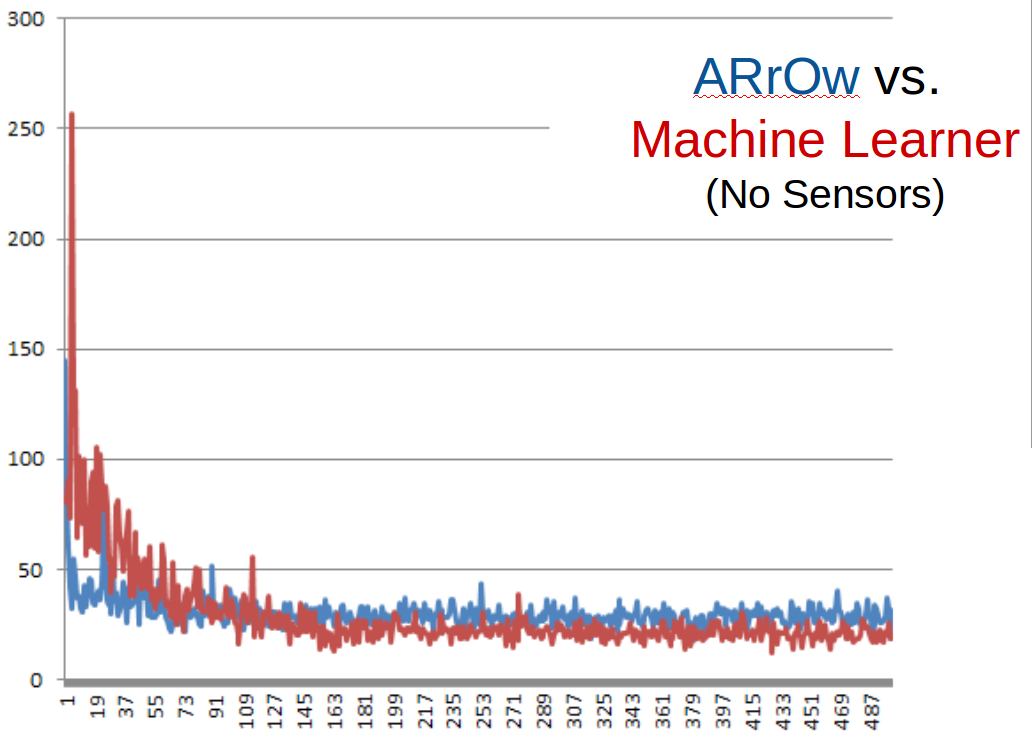
\includegraphics[width=0.9\columnwidth]{BFSMResult.png} % Reduce the figure size so that it is slightly narrower than the column. Don't use precise values for figure width.This setup will avoid overfull boxes. 
  \caption{Agents in the Blind FSM Environment}
  \label{fig4}
\end{figure}

*** TODO: Figure 4 will need to be modified as follows:

***    a) we need to put data from MaRz in there.

***    b) generate more data so we have a smoother curve

***    c) we can't rely on colors as this will be printed in b/w

***    d) generate as a high quality image, preferably in PDF format


Predictably, the number of steps to reach the goal declines
exponential on successive trips the goal indicating that the agent is
learning to improve its behavior.  This is true for all three
algorithms.

Figure \ref{fig5} shows the results for the OSFSM environment.  The scope of
the machine is the same: 50 states, 3 letter alphabet.  

\begin{figure}[t]
  \centering
  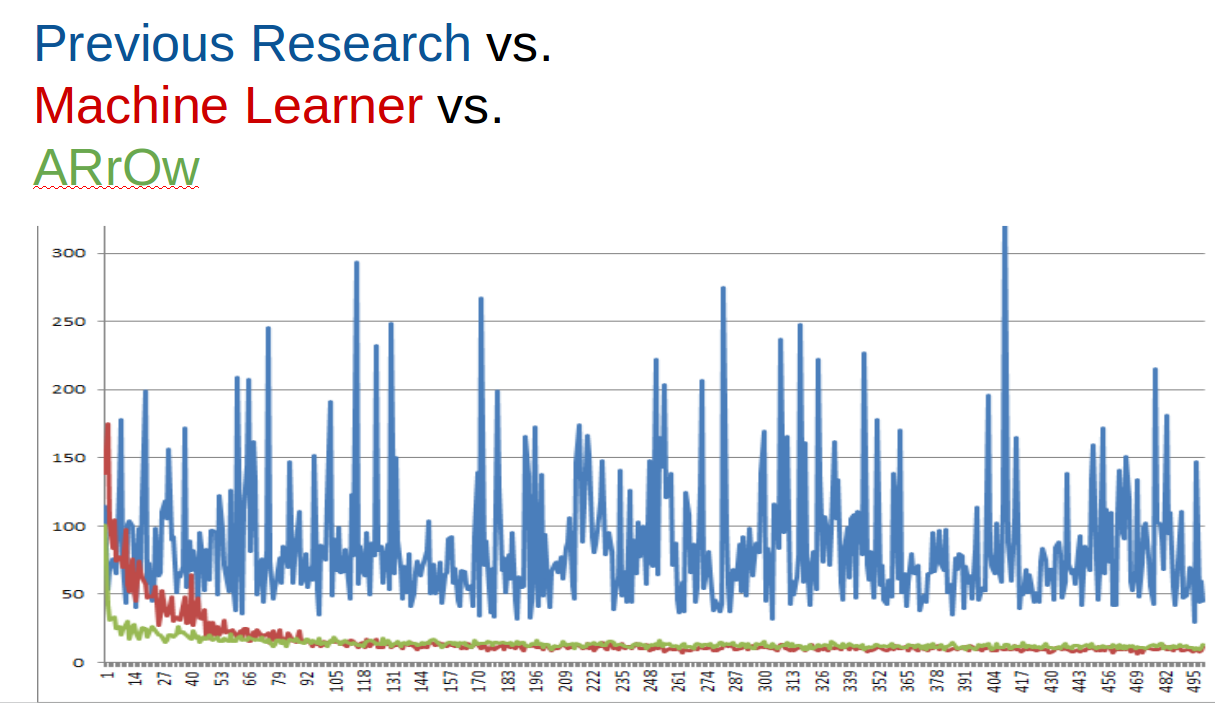
\includegraphics[width=0.9\columnwidth]{OSFSMResult.png} % Reduce the figure size so that it is slightly narrower than the column. Don't use precise values for figure width.This setup will avoid overfull boxes. 
  \caption{Agents in the Odd-Sensor FSM Environment}
  \label{fig5}
\end{figure}

*** TODO: Figure 5 will need to be modified as follows:

***    a) we can't rely on colors as this will be printed in b/w

***    b) generate more data so we have a smoother curve

***    c) generate as a high quality image, preferably in PDF format


As shown, ARO is able to learn near optimal behavior much more rapidly
than the other algorithms.  These results were consistent across a
variety of different machines ranging from [min] to [max] states and
alphabets of [min] to [max] letters.

***TODO:  fill in [min] and [max] above.

\section{Future Work}

This work demonstrates that ARO is effective in two specific
environments with extreme state aliasing.  Future work will be
required to test the algorithm in other environments.

The most pressing concern is that it is not obvious how best to expand
ARO's rule tree to accommodate additional sensors.  The apparent,
possibly naive, approach is to simply increase the branching factor of
the rule tree.  However, this factor increases exponentially as the
number of sensors increases.  It might be preferable to only include
nodes on an as-needed basis or seek ways to discover sensors or sensor
combinations that can be ignored without unduly impairing the agent's
performance.

ARO may also need to be adjusted to address environment with these
properties:
\begin{itemize}
\item a reward function rather than a single goal state
\item a non-deterministic FSM
\item a dynamic transition table
\end{itemize}

\begin{quote}
\begin{small}
\bibliographystyle{aaai}
\bibliography{aro}
\end{small}
\end{quote}



\end{document}
